% Compile with: lualatex diffusion_code_walkthrough.tex
\documentclass[11pt,a4paper]{article}

% Fonts and encoding
\usepackage{fontspec}
\setmainfont{Latin Modern Roman}
\setmonofont{Latin Modern Mono}

% Core packages
\usepackage{amsmath,amssymb,amsfonts}
\usepackage{booktabs}
\usepackage{xcolor}
\usepackage{listings}
\usepackage{geometry}
\usepackage{hyperref}
\usepackage{tikz}
\usetikzlibrary{positioning, arrows.meta}
\usepackage[most]{tcolorbox}
\tcbuselibrary{breakable,skins}
\usepackage{enumitem}

\geometry{margin=1in}

% Colors
\definecolor{codegreen}{rgb}{0,0.6,0}
\definecolor{codegray}{rgb}{0.5,0.5,0.5}
\definecolor{codepurple}{rgb}{0.58,0,0.82}
\definecolor{backcolour}{rgb}{0.97,0.97,0.97}
\definecolor{keywordcolor}{RGB}{0,0,180}
\definecolor{stringcolor}{RGB}{163,21,21}
\definecolor{commentcolor}{RGB}{0,128,0}
\definecolor{mathbox}{RGB}{240,248,255}
\definecolor{stepcolor}{RGB}{70,130,180}

% Code listing style
\lstdefinestyle{python}{
    language=Python,
    backgroundcolor=\color{backcolour},
    commentstyle=\color{commentcolor}\scriptsize,
    keywordstyle=\color{keywordcolor}\bfseries,
    stringstyle=\color{stringcolor},
    basicstyle=\ttfamily\scriptsize,
    breakatwhitespace=false,
    breaklines=true,
    breakautoindent=true,
    prebreak=\raisebox{0ex}[0ex][0ex]{\ensuremath{\hookleftarrow}},
    captionpos=b,
    keepspaces=true,
    numbers=none,
    showspaces=false,
    showstringspaces=false,
    showtabs=false,
    tabsize=2,
    frame=single,
    rulecolor=\color{gray!30},
    morekeywords={self, True, False, None},
    columns=fullflexible,
    basewidth={0.5em,0.4em},
}

\lstset{style=python}

% Math box (breakable across pages)
\newtcolorbox{mathbox}[1][]{
    colback=mathbox,
    colframe=stepcolor,
    boxrule=0.5pt,
    arc=3pt,
    left=6pt,
    right=6pt,
    top=6pt,
    bottom=6pt,
    breakable,
    enhanced,
    #1
}

% Step box (breakable across pages)
\newtcolorbox{stepbox}[2][]{
    colback=white,
    colframe=stepcolor,
    fonttitle=\bfseries,
    title=#2,
    boxrule=1pt,
    arc=3pt,
    left=4pt,
    right=4pt,
    breakable,
    enhanced,
    #1
}

% Narrower listing environment for use inside boxes
\lstnewenvironment{codebox}{%
    \lstset{style=python,xleftmargin=0pt,xrightmargin=0pt}%
}{}

\title{\textbf{GETRegionDiffusion: Code Implementation Walkthrough}\\[0.5em]
\large Mathematical Foundations and PyTorch Implementation}
\author{Technical Documentation}
\date{\today}

\begin{document}

\maketitle

\tableofcontents

\section{Overview}

This document provides a comprehensive walkthrough of the \texttt{GETRegionDiffusion} model implementation, explaining the mathematical foundations behind each component and how they map to PyTorch code.

\subsection{Data Flow}

The complete forward pass follows this pipeline:
\[
\underbrace{\mathbf{X}}_{\text{Input}} \xrightarrow{\text{Embed}} 
\underbrace{\mathbf{H}}_{\text{Hidden}} \xrightarrow{\text{Mask}} 
\underbrace{\tilde{\mathbf{H}}}_{\text{Masked}} \xrightarrow{\text{DiT}} 
\underbrace{\mathbf{Z}}_{\text{Encoded}} \xrightarrow{\text{Head}} 
\underbrace{\hat{\mathbf{X}}}_{\text{Output}}
\]

Where:
\begin{itemize}
    \item $\mathbf{X} \in \mathbb{R}^{B \times N \times M}$: Input motif features ($B$=batch, $N$=900 regions, $M$=283 motifs)
    \item $\mathbf{H} \in \mathbb{R}^{B \times N \times D}$: Embedded features ($D$=768)
    \item $\tilde{\mathbf{H}}$: Features with masked positions replaced
    \item $\mathbf{Z}$: Transformer-encoded features
    \item $\hat{\mathbf{X}}$: Predicted motif features
\end{itemize}

%==============================================================================
\section{Step 1: Region Embedding}
%==============================================================================

\begin{stepbox}{Step 1: RegionEmbed --- Linear Projection}

\textbf{Purpose:} Project raw motif features from input dimension to model dimension.

\begin{mathbox}
\textbf{Mathematical Formulation:}
\[
\mathbf{H} = \mathbf{X} \mathbf{W}_{\text{embed}} + \mathbf{b}_{\text{embed}}
\]
where:
\begin{itemize}[noitemsep]
    \item $\mathbf{X} \in \mathbb{R}^{B \times N \times 283}$ --- input motif features
    \item $\mathbf{W}_{\text{embed}} \in \mathbb{R}^{283 \times 768}$ --- learnable weight matrix
    \item $\mathbf{b}_{\text{embed}} \in \mathbb{R}^{768}$ --- learnable bias
    \item $\mathbf{H} \in \mathbb{R}^{B \times N \times 768}$ --- embedded output
\end{itemize}
\end{mathbox}

\textbf{PyTorch Implementation:}
\begin{lstlisting}
class RegionEmbed(BaseModule):
    def __init__(self, cfg: RegionEmbedConfig):
        super().__init__(cfg)
        self.embed = nn.Linear(cfg.num_features, cfg.embed_dim)
        # Linear(283, 768)

    def forward(self, x, **kwargs):
        x = self.embed(x)  # (B, 900, 283) -> (B, 900, 768)
        return x
\end{lstlisting}

\end{stepbox}

%==============================================================================
\section{Step 2: Masking Operation}
%==============================================================================

\begin{stepbox}{Step 2: Masking + Token Replacement}

\textbf{Purpose:} Replace masked positions with a learnable mask token while preserving unmasked positions.

\begin{mathbox}
\textbf{Mathematical Formulation:}

For each position $i$ in the sequence:
\[
\tilde{\mathbf{h}}_i = \begin{cases}
\mathbf{h}_i & \text{if } m_i = 0 \text{ (unmasked)} \\
\mathbf{e}_{\text{mask}} & \text{if } m_i = 1 \text{ (masked)}
\end{cases}
\]

Vectorized form using element-wise operations:
\[
\tilde{\mathbf{H}} = \mathbf{H} \odot (1 - \mathbf{M}) + \mathbf{E}_{\text{mask}} \odot \mathbf{M}
\]
where:
\begin{itemize}[noitemsep]
    \item $\mathbf{M} \in \{0, 1\}^{B \times N \times 1}$ --- binary mask (broadcast to hidden dim)
    \item $\mathbf{E}_{\text{mask}} \in \mathbb{R}^{B \times N \times D}$ --- mask token expanded to all positions
    \item $\odot$ --- element-wise (Hadamard) product
\end{itemize}
\end{mathbox}

\textbf{PyTorch Implementation:}
\begin{lstlisting}
# In forward():
# mask_token is a learnable parameter: (1, 1, 768)
mask_token = self.mask_token.expand(B, N, -1)  # -> (B, 900, 768)

# Convert boolean mask to float for multiplication
w = mask.type_as(mask_token)  # True->1.0, False->0.0

# keep original where mask=0, use mask_token where mask=1
x = x * (1 - w) + mask_token * w
\end{lstlisting}

\textbf{Token Initialization:}
\begin{lstlisting}
# Learnable tokens initialized with truncated normal distribution
self.mask_token = nn.Parameter(torch.zeros(1, 1, 768))
self.cls_token = nn.Parameter(torch.zeros(1, 1, 768))
trunc_normal_(self.mask_token, std=0.02)
trunc_normal_(self.cls_token, std=0.02)
\end{lstlisting}

\end{stepbox}

%==============================================================================
\section{Step 3: CLS Token Prepending}
%==============================================================================

\begin{stepbox}{Step 3: Add CLS Token}

\textbf{Purpose:} Prepend a learnable classification token to the sequence.

\begin{mathbox}
\textbf{Mathematical Formulation:}
\[
\mathbf{H}' = \text{concat}([\mathbf{e}_{\text{cls}}, \tilde{\mathbf{H}}], \text{dim}=1)
\]
where:
\begin{itemize}[noitemsep]
    \item $\mathbf{e}_{\text{cls}} \in \mathbb{R}^{B \times 1 \times D}$ --- CLS token (expanded to batch)
    \item $\tilde{\mathbf{H}} \in \mathbb{R}^{B \times N \times D}$ --- masked hidden states
    \item $\mathbf{H}' \in \mathbb{R}^{B \times (N+1) \times D}$ --- output with CLS token
\end{itemize}

Sequence length changes: $900 \rightarrow 901$
\end{mathbox}

\textbf{PyTorch Implementation:}
\begin{lstlisting}
# Expand CLS token to batch size
cls_tokens = self.cls_token.expand(B, -1, -1)  # (1,1,768) -> (B,1,768)

# Concatenate along sequence dimension
x = torch.cat((cls_tokens, x), dim=1)  # (B, 901, 768)
\end{lstlisting}

\end{stepbox}

%==============================================================================
\section{Step 4: Timestep Sampling}
%==============================================================================

\begin{stepbox}{Step 4: Random Timestep Sampling}

\textbf{Purpose:} Sample a random diffusion timestep for each batch element.

\begin{mathbox}
\textbf{Mathematical Formulation:}
\[
t \sim \text{Uniform}\{0, 1, 2, \ldots, T-1\}
\]
where $T = 1000$ (number of diffusion timesteps).

Each sample in the batch gets an independent random timestep:
\[
\mathbf{t} = [t_1, t_2, \ldots, t_B] \in \{0, \ldots, 999\}^B
\]
\end{mathbox}

\textbf{PyTorch Implementation:}
\begin{lstlisting}
# Sample random timesteps for each batch element
t = torch.randint(0, self.num_timesteps, (B,), device=device).long()
# t.shape = (B,), e.g., tensor([342, 891, 127, ...])
\end{lstlisting}

\end{stepbox}

%==============================================================================
\section{Step 5: Timestep Embedding}
%==============================================================================

\begin{stepbox}{Step 5: TimestepEmbedder --- Sinusoidal + MLP}

\textbf{Purpose:} Convert scalar timesteps into rich vector representations for conditioning.

\begin{mathbox}
\textbf{Mathematical Formulation:}

\textbf{Stage 1: Sinusoidal Embedding} (same as Transformer positional encoding)

For timestep $t$ and dimension $d = 256$:
\[
\text{PE}(t, 2i) = \sin\left(\frac{t}{\tau^{2i/d}}\right), \quad
\text{PE}(t, 2i+1) = \cos\left(\frac{t}{\tau^{2i/d}}\right)
\]
where $\tau = 10000$ (max period) and $i \in \{0, 1, \ldots, d/2 - 1\}$.

Equivalently:
\[
\omega_i = \exp\left(-\frac{\log(\tau) \cdot i}{d/2}\right), \quad
\mathbf{e}_{\text{freq}}(t) = [\cos(t \cdot \boldsymbol{\omega}), \sin(t \cdot \boldsymbol{\omega})]
\]

\textbf{Stage 2: MLP Projection}
\[
\mathbf{c} = \mathbf{W}_2 \cdot \text{SiLU}(\mathbf{W}_1 \cdot \mathbf{e}_{\text{freq}}(t) + \mathbf{b}_1) + \mathbf{b}_2
\]
where:
\begin{itemize}[noitemsep]
    \item $\mathbf{W}_1 \in \mathbb{R}^{768 \times 256}$, $\mathbf{b}_1 \in \mathbb{R}^{768}$
    \item $\mathbf{W}_2 \in \mathbb{R}^{768 \times 768}$, $\mathbf{b}_2 \in \mathbb{R}^{768}$
    \item $\text{SiLU}(x) = x \cdot \sigma(x)$ where $\sigma$ is sigmoid
    \item $\mathbf{c} \in \mathbb{R}^{B \times 768}$ --- conditioning vector
\end{itemize}
\end{mathbox}

\textbf{PyTorch Implementation:}
\begin{lstlisting}
class TimestepEmbedder(nn.Module):
    def __init__(self, hidden_size, freq_embed_size=256):
        super().__init__()
        self.mlp = nn.Sequential(
            nn.Linear(freq_embed_size, hidden_size),  # 256->768
            nn.SiLU(),
            nn.Linear(hidden_size, hidden_size),      # 768->768
        )
        self.frequency_embedding_size = freq_embed_size

    @staticmethod
    def timestep_embedding(t, dim, max_period=10000):
        half = dim // 2  # 128
        # Frequencies: exp(-log(10000) * [0,...,127] / 128)
        freqs = torch.exp(
            -math.log(max_period) * 
            torch.arange(0, half, dtype=torch.float32) / half
        ).to(device=t.device)
        
        # Outer product: t[:, None] * freqs[None]
        args = t[:, None].float() * freqs[None]
        
        # Concatenate cos and sin -> (B, 256)
        embedding = torch.cat(
            [torch.cos(args), torch.sin(args)], dim=-1)
        return embedding

    def forward(self, t):
        t_freq = self.timestep_embedding(
            t, self.frequency_embedding_size)  # (B, 256)
        t_emb = self.mlp(t_freq)  # (B, 768)
        return t_emb
\end{lstlisting}

\end{stepbox}

%==============================================================================
\section{Step 6: Adaptive Layer Normalization (adaLN)}
%==============================================================================

\begin{stepbox}{Step 6: The \texttt{modulate} Function --- Core of adaLN}

\textbf{Purpose:} Inject timestep conditioning into the transformer by modulating normalized activations.

\begin{mathbox}
\textbf{Standard LayerNorm:}
\[
\text{LN}(\mathbf{x}) = \gamma \odot \frac{\mathbf{x} - \mu}{\sigma} + \beta
\]
where $\gamma, \beta$ are \textbf{fixed} learnable parameters.

\textbf{Adaptive LayerNorm (adaLN):}
\[
\text{adaLN}(\mathbf{x}, \mathbf{c}) = (1 + \text{scale}) \odot \frac{\mathbf{x} - \mu}{\sigma} + \text{shift}
\]
where $\text{scale}, \text{shift}$ are \textbf{predicted from conditioning} $\mathbf{c}$.

\textbf{The modulate function:}
\[
\text{modulate}(\mathbf{x}, \text{shift}, \text{scale}) = \mathbf{x} \odot (1 + \text{scale}) + \text{shift}
\]

Key insight: $(1 + \text{scale})$ ensures identity behavior when $\text{scale} = 0$.
\end{mathbox}

\textbf{PyTorch Implementation:}
\begin{lstlisting}
def modulate(x, shift, scale):
    """
    x: (B, L, D) - input tensor
    shift, scale: (B, D) - modulation parameters from timestep
    Returns: (B, L, D) - modulated tensor
    """
    # unsqueeze(1) broadcasts (B, D) -> (B, 1, D) for sequence dimension
    return x * (1 + scale.unsqueeze(1)) + shift.unsqueeze(1)
\end{lstlisting}

\textbf{Why this works:}
\begin{itemize}
    \item At initialization, adaLN outputs are zero $\Rightarrow$ scale=0, shift=0
    \item $\text{modulate}(\mathbf{x}, 0, 0) = \mathbf{x} \cdot 1 + 0 = \mathbf{x}$ (identity)
    \item Model gradually learns conditioning through training
\end{itemize}

\end{stepbox}

%==============================================================================
\section{Step 7: DiTBlock --- Transformer Block with adaLN}
%==============================================================================

\begin{stepbox}{Step 7: DiTBlock --- The Core Transformer Block}

\textbf{Purpose:} Process sequence with self-attention and feed-forward, conditioned on timestep.

\begin{mathbox}
\textbf{Mathematical Formulation:}

\textbf{Stage 1: Compute 6 modulation parameters from conditioning}
\[
[\gamma_1, \beta_1, \alpha_1, \gamma_2, \beta_2, \alpha_2] = \text{MLP}_{\text{adaLN}}(\mathbf{c})
\]
where MLP$_{\text{adaLN}}$: $\mathbb{R}^{768} \rightarrow \mathbb{R}^{4608}$ (6 $\times$ 768).

\textbf{Stage 2: Self-Attention with gated residual}
\[
\mathbf{x}' = \mathbf{x} + \alpha_1 \odot \text{Attention}\left(\text{modulate}(\text{LN}(\mathbf{x}), \beta_1, \gamma_1)\right)
\]

\textbf{Stage 3: Feed-Forward with gated residual}
\[
\mathbf{x}'' = \mathbf{x}' + \alpha_2 \odot \text{MLP}\left(\text{modulate}(\text{LN}(\mathbf{x}'), \beta_2, \gamma_2)\right)
\]

Where:
\begin{itemize}[noitemsep]
    \item $\gamma_i$ = scale parameters
    \item $\beta_i$ = shift parameters  
    \item $\alpha_i$ = gate parameters (control residual contribution)
    \item LN uses \texttt{elementwise\_affine=False} (no $\gamma, \beta$)
\end{itemize}
\end{mathbox}

\textbf{PyTorch Implementation:}
\begin{lstlisting}
class DiTBlock(nn.Module):
    def __init__(self, hidden_size, num_heads, mlp_ratio=4.0):
        super().__init__()
        # LayerNorm WITHOUT learnable gamma/beta
        self.norm1 = nn.LayerNorm(hidden_size, 
                                  elementwise_affine=False, eps=1e-6)
        self.attn = Attention(hidden_size, num_heads=num_heads, 
                              qkv_bias=True)
        self.norm2 = nn.LayerNorm(hidden_size, 
                                  elementwise_affine=False, eps=1e-6)
        
        mlp_hidden_dim = int(hidden_size * mlp_ratio)  # 3072
        self.mlp = Mlp(in_features=hidden_size, 
                       hidden_features=mlp_hidden_dim)
        
        # Predict 6 modulation parameters from conditioning
        self.adaLN_modulation = nn.Sequential(
            nn.SiLU(),
            nn.Linear(hidden_size, 6 * hidden_size)  # 768->4608
        )

    def forward(self, x, c):
        # c: conditioning vector, shape (B, 768)
        
        # Get 6 modulation vectors, each (B, 768)
        modulation = self.adaLN_modulation(c).chunk(6, dim=1)
        shift_msa, scale_msa, gate_msa = modulation[:3]
        shift_mlp, scale_mlp, gate_mlp = modulation[3:]
        
        # Self-Attention block with gated residual
        normed = modulate(self.norm1(x), shift_msa, scale_msa)
        x = x + gate_msa.unsqueeze(1) * self.attn(normed)
        
        # Feed-Forward block with gated residual
        normed = modulate(self.norm2(x), shift_mlp, scale_mlp)
        x = x + gate_mlp.unsqueeze(1) * self.mlp(normed)
        return x
\end{lstlisting}

\end{stepbox}

%==============================================================================
\section{Step 8: Self-Attention Mechanism}
%==============================================================================

\begin{stepbox}{Step 8: Multi-Head Self-Attention}

\textbf{Purpose:} Allow each position to attend to all other positions in the sequence.

\begin{mathbox}
\textbf{Mathematical Formulation:}

\textbf{Stage 1: Linear projections to Q, K, V}
\[
\mathbf{Q} = \mathbf{X}\mathbf{W}_Q, \quad \mathbf{K} = \mathbf{X}\mathbf{W}_K, \quad \mathbf{V} = \mathbf{X}\mathbf{W}_V
\]
In practice, computed as single fused projection:
\[
[\mathbf{Q}, \mathbf{K}, \mathbf{V}] = \mathbf{X}\mathbf{W}_{QKV}
\]
where $\mathbf{W}_{QKV} \in \mathbb{R}^{768 \times 2304}$.

\textbf{Stage 2: Split into heads}
\[
\mathbf{Q}_h, \mathbf{K}_h, \mathbf{V}_h \in \mathbb{R}^{B \times h \times N \times d_k}
\]
where $h = 12$ heads, $d_k = 768/12 = 64$ per head.

\textbf{Stage 3: Scaled dot-product attention}
\[
\text{Attention}(\mathbf{Q}, \mathbf{K}, \mathbf{V}) = \text{softmax}\left(\frac{\mathbf{Q}\mathbf{K}^\top}{\sqrt{d_k}}\right)\mathbf{V}
\]
Scale factor: $\sqrt{d_k} = \sqrt{64} = 8$.

\textbf{Stage 4: Concatenate heads and project}
\[
\text{MultiHead}(\mathbf{X}) = \text{Concat}(\text{head}_1, \ldots, \text{head}_h)\mathbf{W}_O
\]
where $\mathbf{W}_O \in \mathbb{R}^{768 \times 768}$.
\end{mathbox}

\textbf{PyTorch Implementation:}
\begin{lstlisting}
class Attention(nn.Module):
    def __init__(self, dim, num_heads=8, qkv_bias=False):
        super().__init__()
        self.num_heads = num_heads
        head_dim = dim // num_heads  # 768 // 12 = 64
        self.scale = head_dim ** -0.5  # 1/sqrt(64) = 0.125

        self.qkv = nn.Linear(dim, dim * 3, bias=qkv_bias)  # 768 -> 2304
        self.proj = nn.Linear(dim, dim)  # 768 -> 768

    def forward(self, x):
        B, N, C = x.shape  # (B, 901, 768)
        
        # Compute Q, K, V in one projection
        qkv = self.qkv(x)  # (B, 901, 2304)
        qkv = qkv.reshape(B, N, 3, self.num_heads, 
                          C // self.num_heads)
        # Shape: (B, 901, 3, 12, 64)
        qkv = qkv.permute(2, 0, 3, 1, 4)
        # Shape: (3, B, 12, 901, 64)
        q, k, v = qkv[0], qkv[1], qkv[2]

        # Scaled dot-product attention
        attn = (q @ k.transpose(-2, -1)) * self.scale
        attn = attn.softmax(dim=-1)

        # Apply attention to values
        x = (attn @ v)  # (B, 12, 901, 64)
        x = x.transpose(1, 2).reshape(B, N, C)
        
        # Output projection
        x = self.proj(x)
        return x
\end{lstlisting}

\end{stepbox}

%==============================================================================
\section{Step 9: Feed-Forward Network (MLP)}
%==============================================================================

\begin{stepbox}{Step 9: Two-Layer MLP with GELU Activation}

\textbf{Purpose:} Add non-linear transformations to each position independently.

\begin{mathbox}
\textbf{Mathematical Formulation:}
\[
\text{MLP}(\mathbf{x}) = \mathbf{W}_2 \cdot \text{GELU}(\mathbf{W}_1 \mathbf{x} + \mathbf{b}_1) + \mathbf{b}_2
\]
where:
\begin{itemize}[noitemsep]
    \item $\mathbf{W}_1 \in \mathbb{R}^{3072 \times 768}$ --- expansion layer
    \item $\mathbf{W}_2 \in \mathbb{R}^{768 \times 3072}$ --- compression layer
    \item Expansion ratio = 4 (768 $\rightarrow$ 3072 $\rightarrow$ 768)
\end{itemize}

\textbf{GELU activation:}
\[
\text{GELU}(x) = x \cdot \Phi(x) \approx 0.5x\left(1 + \tanh\left[\sqrt{\frac{2}{\pi}}(x + 0.044715x^3)\right]\right)
\]
where $\Phi(x)$ is the standard Gaussian CDF.
\end{mathbox}

\textbf{PyTorch Implementation:}
\begin{lstlisting}
class Mlp(nn.Module):
    def __init__(self, in_features, hidden_features=None, 
                 out_features=None, act_layer=nn.GELU, drop=0.0):
        super().__init__()
        out_features = out_features or in_features
        hidden_features = hidden_features or in_features
        
        self.fc1 = nn.Linear(in_features, hidden_features)
        self.act = act_layer()  # GELU
        self.fc2 = nn.Linear(hidden_features, out_features)
        self.drop = nn.Dropout(drop)

    def forward(self, x):
        x = self.fc1(x)   # 768 -> 3072
        x = self.act(x)   # GELU activation
        x = self.fc2(x)   # 3072 -> 768
        x = self.drop(x)
        return x
\end{lstlisting}

\end{stepbox}

%==============================================================================
\section{Step 10: DiT Encoder Assembly}
%==============================================================================

\begin{stepbox}{Step 10: GETRegionDiTEncoder --- Stacking 12 Blocks}

\textbf{Purpose:} Combine TimestepEmbedder and 12 DiTBlocks into a complete encoder.

\begin{mathbox}
\textbf{Mathematical Formulation:}

\textbf{Complete forward pass:}
\begin{align}
\mathbf{c} &= \text{TimestepEmbedder}(t) \\
\mathbf{h}^{(0)} &= \mathbf{H}' \quad \text{(input with CLS token)} \\
\mathbf{h}^{(\ell)} &= \text{DiTBlock}^{(\ell)}(\mathbf{h}^{(\ell-1)}, \mathbf{c}) \quad \text{for } \ell = 1, \ldots, 12 \\
\mathbf{Z} &= \text{LayerNorm}(\mathbf{h}^{(12)})
\end{align}

Note: The same conditioning vector $\mathbf{c}$ is used for all 12 blocks.
\end{mathbox}

\textbf{PyTorch Implementation:}
\begin{lstlisting}
class GETRegionDiTEncoder(nn.Module):
    def __init__(self, embed_dim=768, depth=12, num_heads=12, mlp_ratio=4.0):
        super().__init__()
        
        # Timestep embedding
        self.t_embedder = TimestepEmbedder(embed_dim)  # 768

        # Stack of 12 DiT blocks
        self.blocks = nn.ModuleList([
            DiTBlock(embed_dim, num_heads, mlp_ratio=mlp_ratio)
            for _ in range(depth)  # 12 blocks
        ])

        # Final LayerNorm (with affine params for output)
        self.norm = nn.LayerNorm(embed_dim, eps=1e-6)

    def forward(self, x, t):
        """
        x: (B, 901, 768) - embedded regions with CLS
        t: (B,) - timestep indices
        """
        # Convert timestep to conditioning vector
        c = self.t_embedder(t)  # (B, 768)

        # Pass through all DiT blocks
        for blk in self.blocks:
            x = blk(x, c)  # Same c for all blocks

        # Final normalization
        x = self.norm(x)  # (B, 901, 768)
        return x
\end{lstlisting}

\textbf{Critical: Zero Initialization for Stability}
\begin{lstlisting}
def initialize_weights(self):
    # ... standard init ...
    
    # Zero-out adaLN layers for identity initialization
    for block in self.blocks:
        nn.init.constant_(block.adaLN_modulation[-1].weight, 0)
        nn.init.constant_(block.adaLN_modulation[-1].bias, 0)
\end{lstlisting}

This ensures $\text{scale} = \text{shift} = \text{gate} = 0$ at init, so:
\begin{itemize}
    \item $\text{modulate}(\mathbf{x}, 0, 0) = \mathbf{x}$ (identity)
    \item $\text{gate} \cdot \text{output} = 0$ (no residual contribution)
\end{itemize}

\end{stepbox}

%==============================================================================
\section{Step 11: CLS Token Removal \& Prediction Head}
%==============================================================================

\begin{stepbox}{Step 11: Output Processing}

\textbf{Purpose:} Remove CLS token and project back to motif space.

\begin{mathbox}
\textbf{Mathematical Formulation:}

\textbf{Stage 1: Remove CLS token}
\[
\mathbf{Z}_{\text{regions}} = \mathbf{Z}[:, 1:, :] \in \mathbb{R}^{B \times N \times D}
\]
(Remove first token, keep positions 1 to 900)

\textbf{Stage 2: Linear projection to output}
\[
\hat{\mathbf{X}} = \mathbf{Z}_{\text{regions}} \mathbf{W}_{\text{head}} + \mathbf{b}_{\text{head}}
\]
where:
\begin{itemize}[noitemsep]
    \item $\mathbf{W}_{\text{head}} \in \mathbb{R}^{768 \times 283}$
    \item $\hat{\mathbf{X}} \in \mathbb{R}^{B \times 900 \times 283}$ --- predicted motif features
\end{itemize}
\end{mathbox}

\textbf{PyTorch Implementation:}
\begin{lstlisting}
# In forward():
# After encoder
x = self.encoder(x, t)  # (B, 901, 768)

# Remove CLS token (index 0)
x = x[:, 1:]  # (B, 900, 768)

# Project to output dimension
x_masked = self.head_mask(x)  # (B, 900, 283)

# head_mask is defined as:
self.head_mask = nn.Linear(768, 283)  # in_features, out_features from config
\end{lstlisting}

\end{stepbox}

%==============================================================================
\section{Step 12: Loss Computation}
%==============================================================================

\begin{stepbox}{Step 12: Masked MSE Loss}

\textbf{Purpose:} Compute reconstruction loss only on masked positions.

\begin{mathbox}
\textbf{Mathematical Formulation:}
\[
\mathcal{L} = \frac{1}{|\mathcal{M}|} \sum_{i \in \mathcal{M}} \|\hat{\mathbf{x}}_i - \mathbf{x}_i\|_2^2
\]
where:
\begin{itemize}[noitemsep]
    \item $\mathcal{M} = \{i : m_i = 1\}$ --- set of masked indices
    \item $\hat{\mathbf{x}}_i \in \mathbb{R}^{283}$ --- predicted motif vector at position $i$
    \item $\mathbf{x}_i \in \mathbb{R}^{283}$ --- ground truth motif vector
\end{itemize}

\textbf{Implementation trick:} Zero out unmasked positions before loss:
\[
\text{pred}_{\text{masked}} = \hat{\mathbf{X}} \odot \mathbf{M}, \quad
\text{target}_{\text{masked}} = \mathbf{X} \odot \mathbf{M}
\]
Then MSE naturally ignores zeros (they contribute 0 to loss).
\end{mathbox}

\textbf{PyTorch Implementation:}
\begin{lstlisting}
def before_loss(self, output, batch):
    """Prepare predictions and targets for loss computation."""
    x_masked, x_original, mask = output
    
    # Apply mask to both predictions and targets
    # Masked positions: compute loss
    # Unmasked positions: multiply by 0 (ignore)
    pred = {'masked': x_masked * mask}    # (B, 900, 283) * (B, 900, 1)
    obs = {'masked': x_original * mask}
    
    return pred, obs

# Loss is then computed as:
# loss = MSELoss(pred['masked'], obs['masked'])
\end{lstlisting}

\textbf{From config (dit.yaml):}
\begin{lstlisting}
loss:
  components:
    masked:
      _target_: torch.nn.MSELoss
      reduction: mean
  weights:
    masked: 1.0
\end{lstlisting}

\end{stepbox}

%==============================================================================
\section{Step 13: Diffusion Schedule}
%==============================================================================

\begin{stepbox}{Step 13: Noise Schedule Setup}

\textbf{Purpose:} Precompute diffusion noise schedule parameters.

\begin{mathbox}
\textbf{Mathematical Formulation:}

\textbf{Linear beta schedule:}
\[
\beta_t = \beta_{\text{start}} + \frac{t}{T-1}(\beta_{\text{end}} - \beta_{\text{start}})
\]
with $\beta_{\text{start}} = 0.0001$, $\beta_{\text{end}} = 0.02$, $T = 1000$.

\textbf{Derived quantities:}
\begin{align}
\alpha_t &= 1 - \beta_t \\
\bar{\alpha}_t &= \prod_{s=1}^{t} \alpha_s \quad \text{(cumulative product)} \\
\sqrt{\bar{\alpha}_t} &\quad \text{(for signal scaling)} \\
\sqrt{1 - \bar{\alpha}_t} &\quad \text{(for noise scaling)}
\end{align}

\textbf{Forward diffusion process:}
\[
\mathbf{x}_t = \sqrt{\bar{\alpha}_t} \mathbf{x}_0 + \sqrt{1 - \bar{\alpha}_t} \boldsymbol{\epsilon}, \quad \boldsymbol{\epsilon} \sim \mathcal{N}(0, \mathbf{I})
\]
\end{mathbox}

\textbf{PyTorch Implementation:}
\begin{lstlisting}
def _setup_diffusion(self, diff_cfg):
    """Setup noise schedule for diffusion."""
    num_timesteps = diff_cfg.get('num_timesteps', 1000)
    beta_start = diff_cfg.get('beta_start', 0.0001)
    beta_end = diff_cfg.get('beta_end', 0.02)
    
    # Linear schedule: [0.0001, ..., 0.02]
    betas = torch.linspace(beta_start, beta_end, num_timesteps)
    alphas = 1.0 - betas  # alpha_t = 1 - beta_t
    
    # Cumulative product: alpha_bar_t
    alphas_cumprod = torch.cumprod(alphas, dim=0)
    
    # Register as buffers (non-trainable)
    self.register_buffer('betas', betas)
    self.register_buffer('alphas', alphas)
    self.register_buffer('alphas_cumprod', alphas_cumprod)
    self.register_buffer('sqrt_alphas_cumprod', 
                         torch.sqrt(alphas_cumprod))
    self.register_buffer('sqrt_one_minus_alphas_cumprod', 
                         torch.sqrt(1.0 - alphas_cumprod))
    self.num_timesteps = num_timesteps
\end{lstlisting}

\end{stepbox}

%==============================================================================
\section{Complete Forward Pass Summary}
%==============================================================================

\begin{figure}[htbp]
\centering
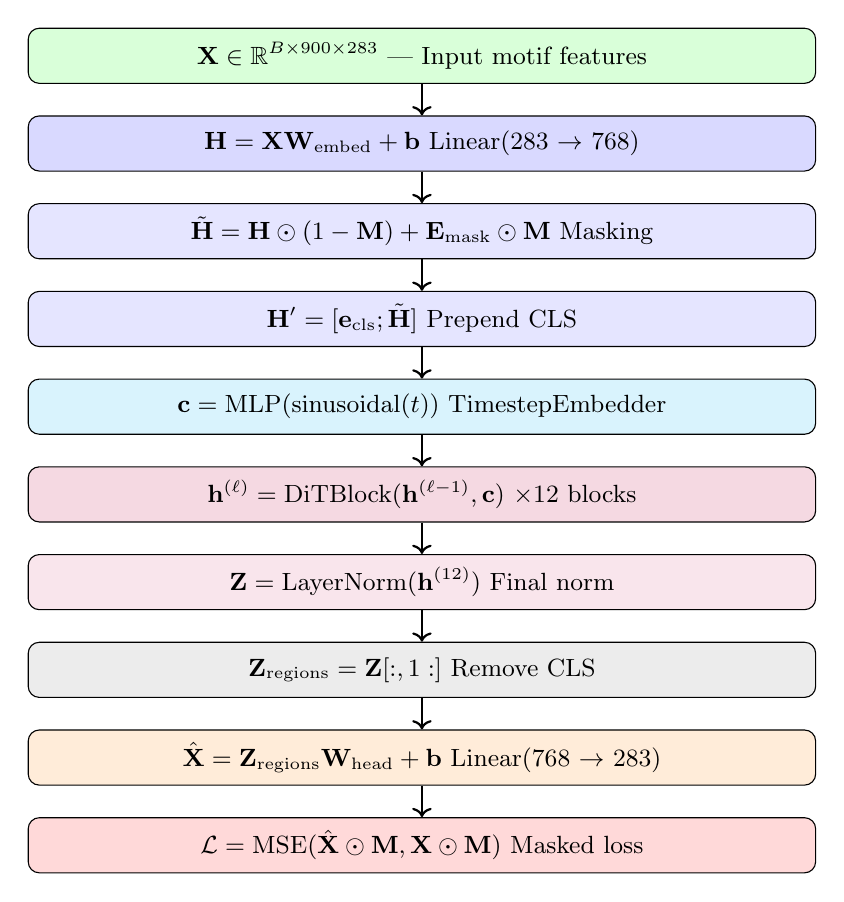
\begin{tikzpicture}[
    node distance=0.4cm,
    box/.style={rectangle, draw, rounded corners, minimum width=10cm, minimum height=0.7cm, align=center, font=\small, fill=#1},
    arrow/.style={->, thick},
]

\node[box=green!15] (input) {$\mathbf{X} \in \mathbb{R}^{B \times 900 \times 283}$ --- Input motif features};
\node[box=blue!15, below=of input] (embed) {$\mathbf{H} = \mathbf{X}\mathbf{W}_{\text{embed}} + \mathbf{b}$ \hfill Linear(283 $\rightarrow$ 768)};
\node[box=blue!10, below=of embed] (mask) {$\tilde{\mathbf{H}} = \mathbf{H} \odot (1-\mathbf{M}) + \mathbf{E}_{\text{mask}} \odot \mathbf{M}$ \hfill Masking};
\node[box=blue!10, below=of mask] (cls) {$\mathbf{H}' = [\mathbf{e}_{\text{cls}}; \tilde{\mathbf{H}}]$ \hfill Prepend CLS};
\node[box=cyan!15, below=of cls] (time) {$\mathbf{c} = \text{MLP}(\text{sinusoidal}(t))$ \hfill TimestepEmbedder};
\node[box=purple!15, below=of time] (dit) {$\mathbf{h}^{(\ell)} = \text{DiTBlock}(\mathbf{h}^{(\ell-1)}, \mathbf{c})$ \hfill $\times 12$ blocks};
\node[box=purple!10, below=of dit] (norm) {$\mathbf{Z} = \text{LayerNorm}(\mathbf{h}^{(12)})$ \hfill Final norm};
\node[box=gray!15, below=of norm] (remove) {$\mathbf{Z}_{\text{regions}} = \mathbf{Z}[:, 1:]$ \hfill Remove CLS};
\node[box=orange!15, below=of remove] (head) {$\hat{\mathbf{X}} = \mathbf{Z}_{\text{regions}}\mathbf{W}_{\text{head}} + \mathbf{b}$ \hfill Linear(768 $\rightarrow$ 283)};
\node[box=red!15, below=of head] (loss) {$\mathcal{L} = \text{MSE}(\hat{\mathbf{X}} \odot \mathbf{M}, \mathbf{X} \odot \mathbf{M})$ \hfill Masked loss};

\foreach \a/\b in {input/embed, embed/mask, mask/cls, cls/time, time/dit, dit/norm, norm/remove, remove/head, head/loss} {
    \draw[arrow] (\a) -- (\b);
}

\end{tikzpicture}
\caption{Complete forward pass with mathematical operations at each step.}
\end{figure}

%==============================================================================
\section{Parameter Count}
%==============================================================================

\begin{table}[htbp]
\centering
\caption{Approximate parameter count for GETRegionDiffusion}
\begin{tabular}{@{}llr@{}}
\toprule
\textbf{Component} & \textbf{Computation} & \textbf{Parameters} \\
\midrule
RegionEmbed & $283 \times 768 + 768$ & 217,856 \\
TimestepEmbedder & $256 \times 768 + 768 + 768 \times 768 + 768$ & 787,968 \\
DiTBlock ($\times 12$) & & \\
\quad - qkv & $768 \times 2304 + 2304$ & 1,771,776 \\
\quad - proj & $768 \times 768 + 768$ & 590,592 \\
\quad - MLP fc1 & $768 \times 3072 + 3072$ & 2,362,368 \\
\quad - MLP fc2 & $3072 \times 768 + 768$ & 2,360,064 \\
\quad - adaLN & $768 \times 4608 + 4608$ & 3,543,552 \\
\quad Subtotal per block & & 10,628,352 \\
\quad All 12 blocks & & 127,540,224 \\
Final LayerNorm & $768 \times 2$ & 1,536 \\
head\_mask & $768 \times 283 + 283$ & 217,627 \\
Tokens (mask + cls) & $768 \times 2$ & 1,536 \\
\midrule
\textbf{Total} & & $\approx$ \textbf{129M} \\
\bottomrule
\end{tabular}
\end{table}

\end{document}

